\documentclass[12pt, a4paper]{article}
\usepackage[utf8]{inputenc}
\usepackage{graphicx}
\usepackage{parskip}
\usepackage{fullpage}

% Opening
\title{Product User Manual}
\author{Team NASA}
\date{}

\begin{document}
\maketitle

\tableofcontents
\pagebreak

\section{Introduction}
Chess is a strategic board game for two players. It is played on a square board consisting of 64 black and white tiles. Each player has a set of playing pieces:
\begin{itemize}
\item King (1)
\item Queen (1)
\item Knights (2)
\item Bishops (2)
\item Rooks (2)
\item Pawns (8)
\end{itemize}

Each of these pieces have rules for how they can move. The end goal of the game is to “checkmate” the other players’ king. This happens when the king cannot escape capture. As in most board games the players take turns in moving their pieces. The first move is made by the player playing the white pieces. The game continues until either; a player resigns, a player gets checkmated or a draw situation occurs.

The game is played around the world by millions of people in all ages. The term “easy to learn, hard to master” fits perfectly for chess, and may be why it is so popular. The game is thought to have originated in India several hundred years ago. The fact that it is still so actively played to this day should be a clear indication of how inducing the game can be.

Target age: 4+

\section{Rules of Chess}

\subsection{Capturing Pieces}
Any chess piece may capture an opposing piece by moving (legally) into the square the other piece currently occupies. A captured piece is removed from the chessboard for the rest of the game.

\subsection{The Chess Pieces}
There are six different types of pieces in chess. They all move in specific ways, and they have unique properties.

\begin{itemize}
\item The pawn: There are eight pawns in a set. With two exceptions, each pawn may only move one square at a time, and only towards the far end of the board – toward the other player. The first exception is if it has not yet moved – in that case, it may move two squares ahead. The second is when a pawn captures another piece. This can only happen by moving the pawn one square forward diagonally into a square occupied by an opposing piece. A pawn cannot move through other pieces. Pawns may partake in two special moves, namely promotion and en passant (see the “Special rules” section below).
\item The rook: There are two rooks in a set. This piece can only move in straight lines, and cannot move through other pieces. A rook, along with the king, may partake in a special move called castling (see “Special rules” below).
\item The knight: There are two knights in a set. A knight can only move in an L-shape: One square horizontally and two squares vertically, or two squares horizontally and one square vertically. It is the only piece with the ability to move through spaces occupied by other pieces.
\item The bishop: There are two bishops in a set. A bishop can only move diagonally, and cannot move through other pieces.
\item The queen: There is one queen in a set. A queen behaves like a combination of a rook and a bishop; it may move any number of squares in a straight or diagonal line. It cannot move through obstructions.
\item The king: There is one king in a set. It may move one square at a time in any direction, and cannot move to an occupied space, except for when capturing an opposing piece. The king, along with a rook, may partake in a special move called castling (see the “Special rules” section below).
 
\begin{itemize}
\item The king is the most important piece in the set, as the game ends when it is captured. It is in check when it is in danger of being captured – meaning an opposing piece could use the following move to attack directly. Letting the king stay in check is illegal; the player must attempt to remove the king from danger as their next move. Checkmate occurs when there are no available legal moves to escape check. 
\end{itemize}
\end{itemize}

\subsection{Setup}
The game is played on a chessboard: A checkered 8x8 square board with alternating light and dark colored tiles. The players are seated opposite to each other.

In this game, there are two kinds of setups available: Standard and Chess960.

\subsubsection{Standard Setup} 
In the standard (and most common) setup, the pieces are placed as follows.

From each player’s perspective, their non-pawn pieces are placed on the closest row in the following order: Rook, knight, bishop, queen or king, queen or king, bishop, knight, rook. The queen is placed on the tile between the bishops that is the same color as itself; for instance, a black queen is always initially placed on a dark tile. The king is placed on the remaining tile on the row. The pawns are placed on the row that is second-closest to the player whose set they belong to.

\subsubsection{Chess960}

Chess960, also called Fischer Random Chess, is a chess variant where the setup differs from standard chess. The non-pawn pieces are placed on the same rank as in the standard setup, but their positions on that rank are randomized.

\subsection{Special Rules}
\begin{itemize}
\item Promotion: If a pawn reaches the opposite end of the board, it can be promoted to the choice of one of the following pieces: A queen, knight, bishop or rook.
\item En passant: This move entails a pawn capture that can only happen immediately after a pawn moves two squares away from its starting point. It can only be performed by an opposing pawn that captures the first pawn “in passing”, meaning the opposing pawn would have been able to capture the first pawn had the latter only moved one square forward.
\item Castling: Once every game, the player may move their king and one of their rooks at the same time. It is considered a king move. Castling entails moving the king two squares to the right or the left (toward the chosen rook), and moving the rook to the last square the king crossed. This move is only legal under the following conditions:	
\begin{itemize}
\item Neither piece has moved previously.
\item There are no pieces between the king and the rook.
\item The king is not in check, and will not pass through or end up on any square under attack by opposing pieces.
\end{itemize}
\end{itemize}

\subsection{How to Win}
A player wins by capturing the other player’s king in a checkmate. It is also possible for a player to win if the opponent resigns.

However, a game of chess can end without a victory – it may end in a draw. For instance, a stalemate occurs when a player is not in check, yet cannot make a legal move. 

\newpage
\section{Key Features of the Game}
\begin{itemize}
\item The user can choose to play against another human player or a machine player with three possible levels of intelligence: Easy, intermediate or hard.
\item The user can choose between various game modes: Regular, rapid, blitz, bullet and Chess960.
\item The user can choose to play against another human player by means of online multiplayer.
\item The user can choose to get a hint describing a tactically sound move.
\item The user can choose to undo the previous move.
\item The user can create an account with a unique username.
\item The program keeps track of the results of each game in a database, and provides an overview of the ranking of players based on how many matches they have won.
\item The program has a 2D chessboard with visually appealing pieces and board layouts that follow standard rules of chess.
\end{itemize}

\newpage
\vfill
\section{Illustrations}
\subsection{Menus}
\begin{figure}[ht!]
	\centering
	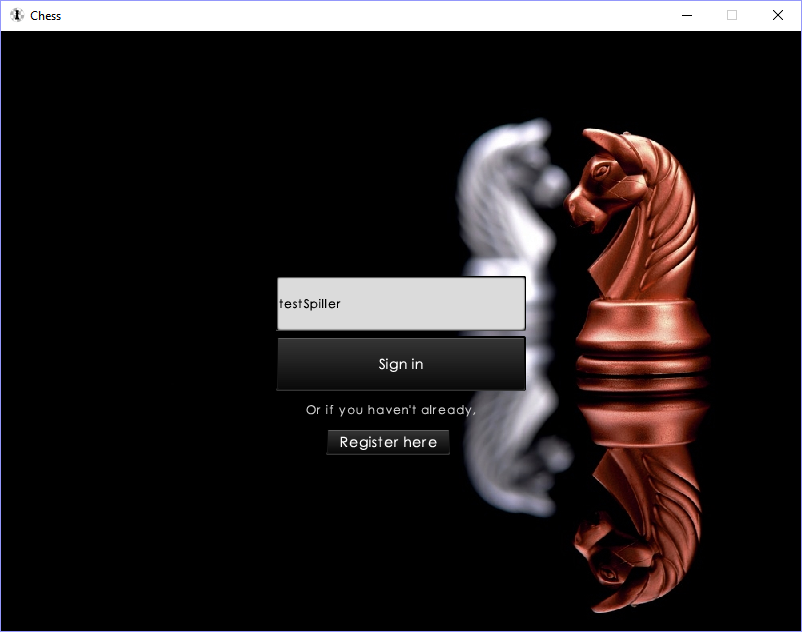
\includegraphics[width=0.725\linewidth]{figures/welcome.png}
	\caption{Welcome screen.}
\end{figure}
\begin{figure}[ht!]
	\centering
	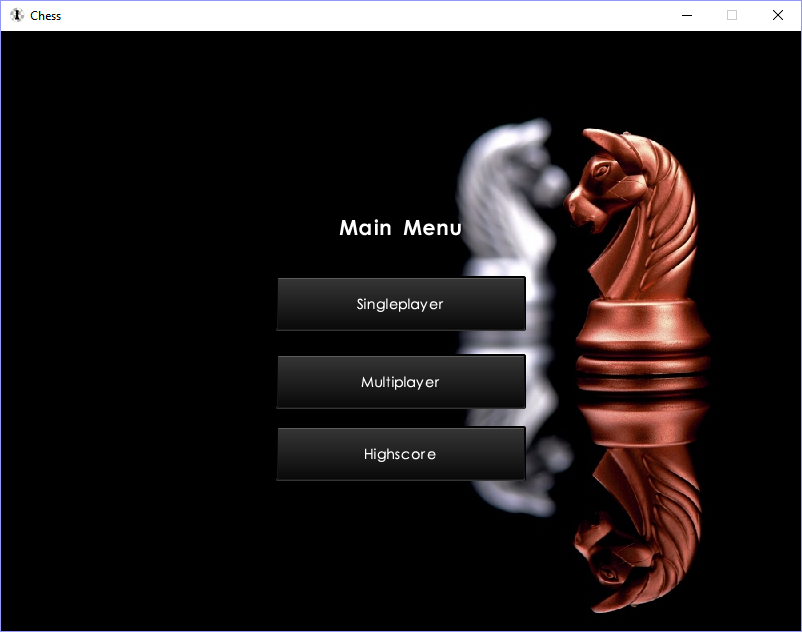
\includegraphics[width=0.725\linewidth]{figures/mainmenu.png}
	\caption{Main menu.}
\end{figure}
\begin{figure}[ht!]
	\centering
	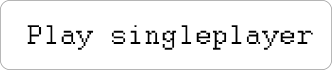
\includegraphics[width=0.8\linewidth]{figures/singleplayer.png}
	\caption{Singleplayer menu.}
\end{figure}
\begin{figure}[ht!]
	\centering
	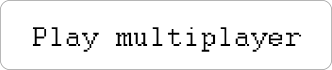
\includegraphics[width=0.8\linewidth]{figures/multiplayer.png}
	\caption{Multiplayer menu.}
\end{figure}
\begin{figure}[ht!]
	\centering
	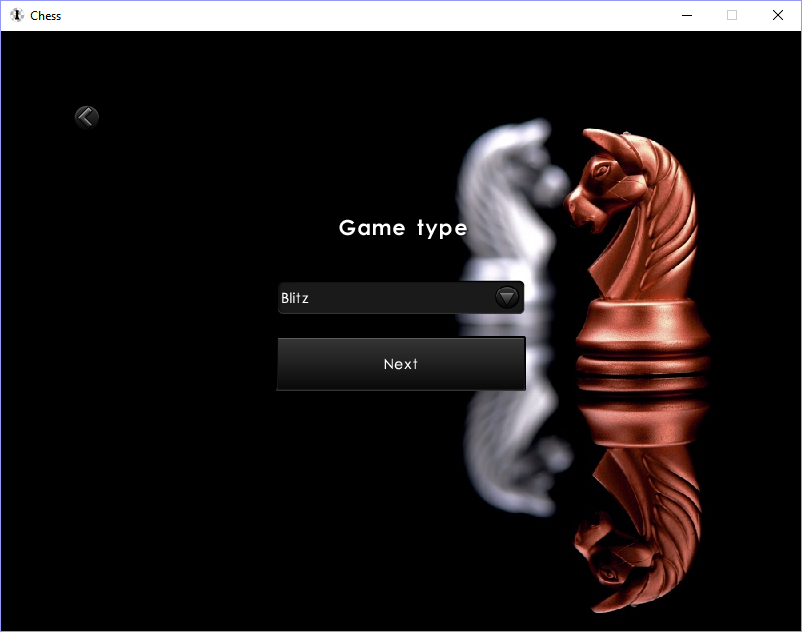
\includegraphics[width=0.8\linewidth]{figures/offline.png}
	\caption{Offline multiplayer.}
\end{figure}
\begin{figure}[ht!]
	\centering
	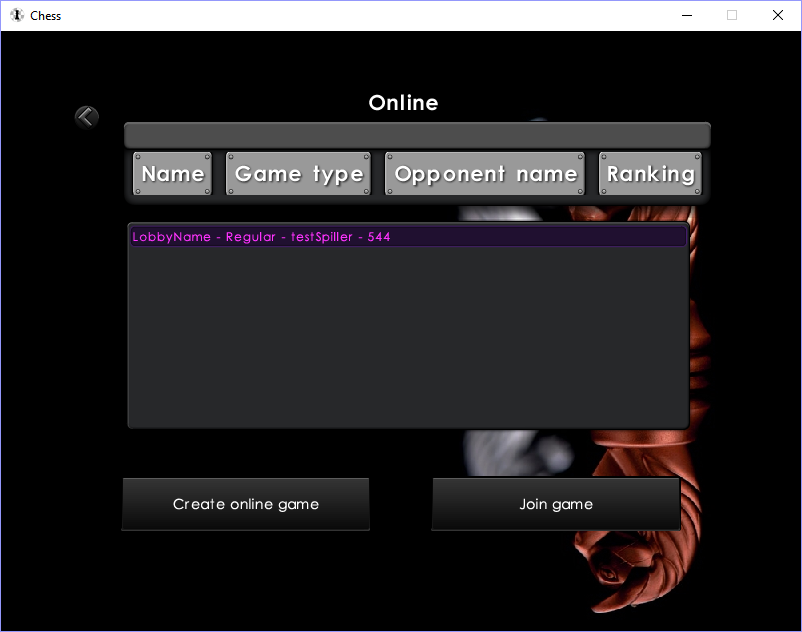
\includegraphics[width=0.8\linewidth]{figures/online.png}
	\caption{Online multiplayer.}
\end{figure}

\newpage
\vfill
\subsection{The Game}
\begin{figure}[ht!]
	\centering
	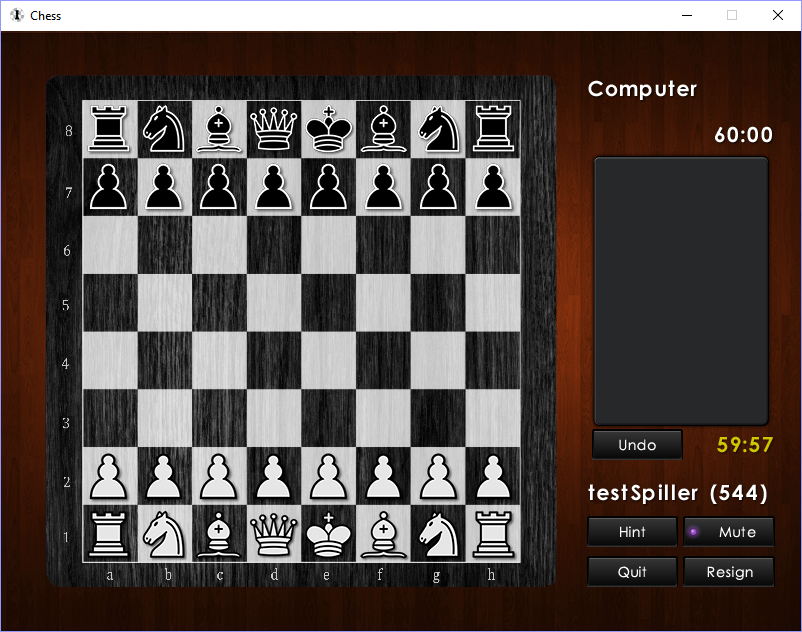
\includegraphics[width=0.725\linewidth]{figures/standard.png}
	\caption{Standard setup.}
\end{figure}
\begin{figure}[ht!]
	\centering
	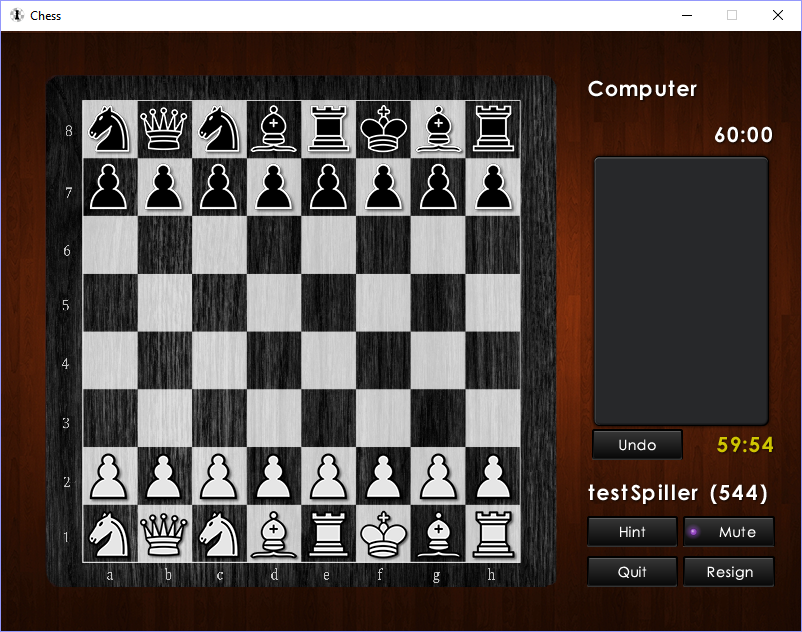
\includegraphics[width=0.725\linewidth]{figures/chess960.png}
	\caption{Chess960 setup.}
\end{figure}
\begin{figure}[ht!]
    \centering
	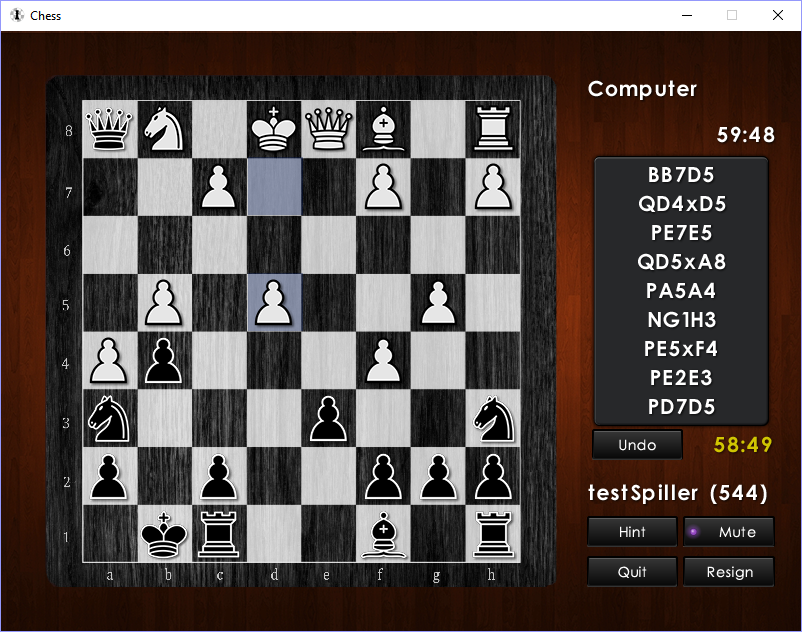
\includegraphics[width=0.8\linewidth]{figures/black.png}
	\caption{Black player one.}
\end{figure}
\begin{figure}[ht!]
	\centering
	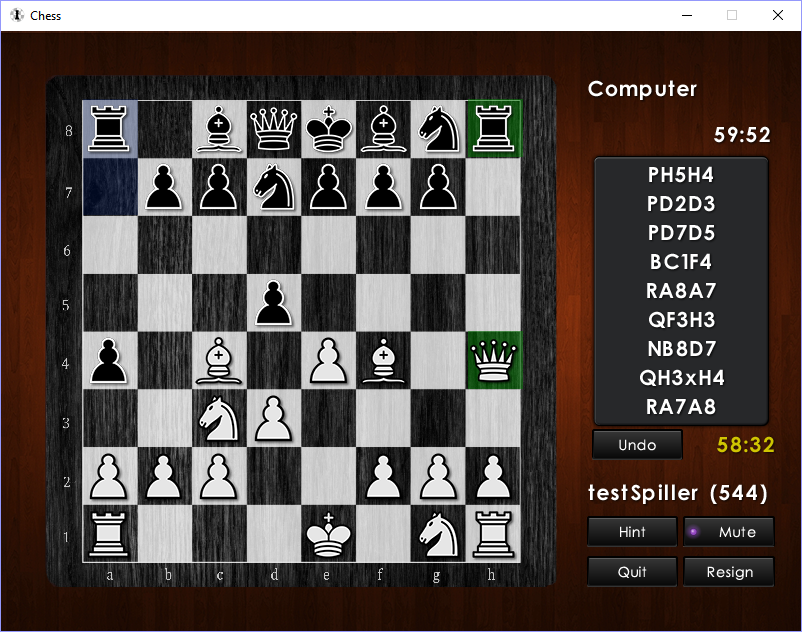
\includegraphics[width=0.8\linewidth]{figures/hint.png}
	\caption{Hint requested.}
\end{figure}
\begin{figure}[ht!]
	\centering
	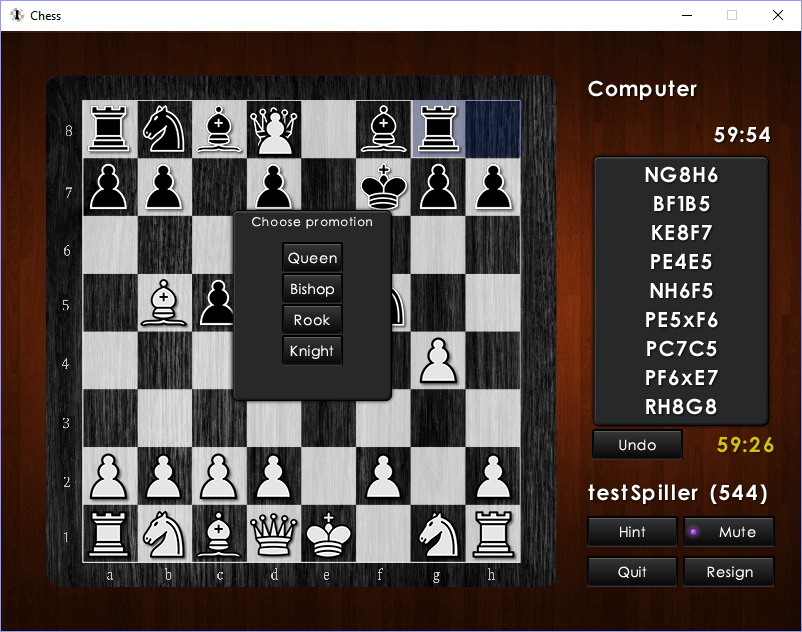
\includegraphics[width=0.8\linewidth]{figures/promotion.png}
	\caption{Pawn promotion prompt.}
\end{figure}
\begin{figure}[ht!]
	\centering
	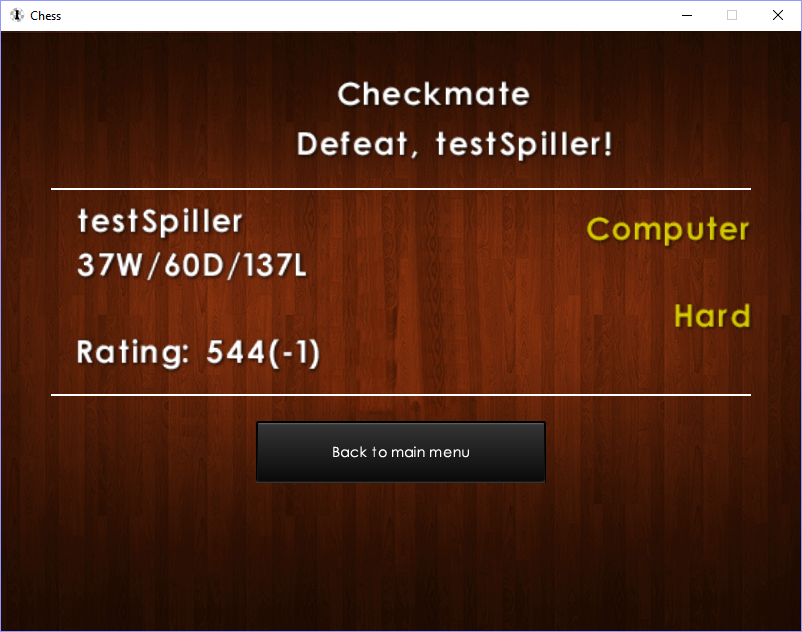
\includegraphics[width=0.8\linewidth]{figures/defeat.png}
	\caption{Defeat.}
\end{figure}
\begin{figure}[ht!]
	\centering
	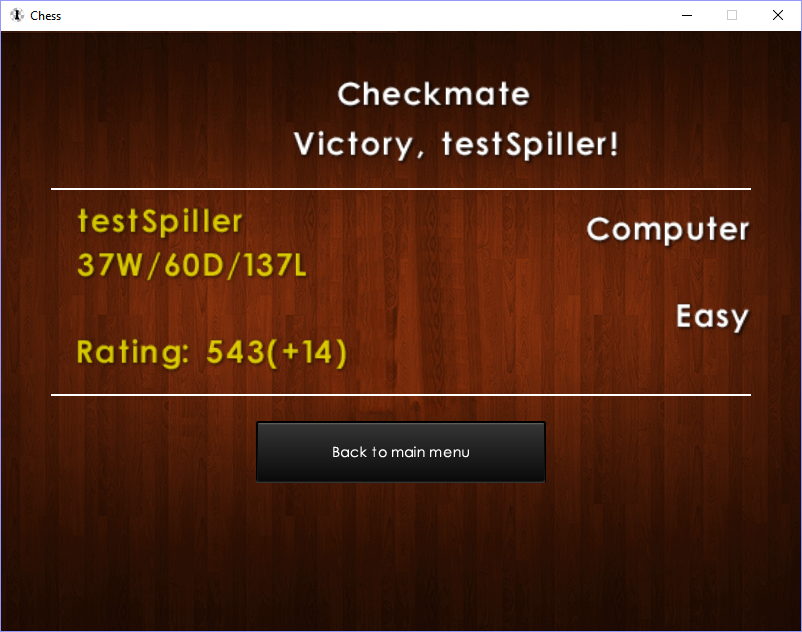
\includegraphics[width=0.8\linewidth]{figures/victory.png}
	\caption{Victory.}
\end{figure}

\end{document}